%%
%% This is file `sample-sigconf.tex',
%% generated with the docstrip utility.
%%
%% The original source files were:
%%
%% samples.dtx  (with options: `sigconf')
%% 
%% IMPORTANT NOTICE:
%% 
%% For the copyright see the source file.
%% 
%% Any modified versions of this file must be renamed
%% with new filenames distinct from sample-sigconf.tex.
%% 
%% For distribution of the original source see the terms
%% for copying and modification in the file samples.dtx.
%% 
%% This generated file may be distributed as long as the
%% original source files, as listed above, are part of the
%% same distribution. (The sources need not necessarily be
%% in the same archive or directory.)
%%
%% The first command in your LaTeX source must be the \documentclass command.
\documentclass[sigconf]{acmart}
%%%% As of March 2017, [siggraph] is no longer used. Please use sigconf (above) for SIGGRAPH conferences.

%%%% Proceedings format for SIGPLAN conferences 
% \documentclass[sigplan, anonymous, review]{acmart}

%%%% Proceedings format for SIGCHI conferences
% \documentclass[sigchi, review]{acmart}

%%%% To use the SIGCHI extended abstract template, please visit
% https://www.overleaf.com/read/zzzfqvkmrfzn

%%
%% \BibTeX command to typeset BibTeX logo in the docs

% Use the postscript times font!
\usepackage{times}
\usepackage{natbib}

\renewcommand*\ttdefault{txtt}
\usepackage{soul}
\usepackage{url}
%\usepackage[hidelinks]{hyperref}
\usepackage[utf8]{inputenc}
\usepackage{graphicx}
\usepackage[small]{subcaption}
\usepackage{amsmath,amssymb,amsthm}
\usepackage{algorithm}
\usepackage[noend]{algorithmic}
\usepackage{booktabs}
\usepackage{multirow}
\usepackage[english]{babel}
\newtheorem{proposition}{\textbf{Proposition}}
\def\BibTeX{{\rm B\kern-.05em{\sc i\kern-.025em b}\kern-.08em
    T\kern-.1667em\lower.7ex\hbox{E}\kern-.125emX}}
\urlstyle{same}

%%
%% \BibTeX command to typeset BibTeX logo in the docs
\AtBeginDocument{%
  \providecommand\BibTeX{{%
    \normalfont B\kern-0.5em{\scshape i\kern-0.25em b}\kern-0.8em\TeX}}}

%% Rights management information.  This information is sent to you
%% when you complete the rights form.  These commands have SAMPLE
%% values in them; it is your responsibility as an author to replace
%% the commands and values with those provided to you when you
%% complete the rights form.
\setcopyright{acmcopyright}
\copyrightyear{2020}
\acmYear{2020}
\acmDOI{10.1145/1122445.1122456}

%% These commands are for a PROCEEDINGS abstract or paper.
\acmConference[San Diego '20]{San Diego '20: ACM Conference on Knowledge, Discovery and Data Mining}{August 22--27, 2020}{San Diego, CA}
\acmBooktitle{San Diego '20: ACM Conference on Knowledge, Discovery and Data Mining, August 22--27, 2020, San Diego, CA}
\acmPrice{15.00}
\acmISBN{978-1-4503-XXXX-X/18/06}


%%
%% Submission ID.
%% Use this when submitting an article to a sponsored event. You'll
%% receive a unique submission ID from the organizers
%% of the event, and this ID should be used as the parameter to this command.
%%\acmSubmissionID{123-A56-BU3}

%%
%% The majority of ACM publications use numbered citations and
%% references.  The command \citestyle{authoryear} switches to the
%% "author year" style.
%%
%% If you are preparing content for an event
%% sponsored by ACM SIGGRAPH, you must use the "author year" style of
%% citations and references.
%% Uncommenting
%% the next command will enable that style.
%%\citestyle{acmauthoryear}

%%
%% end of the preamble, start of the body of the document source.
\begin{document}


\title{Creating Realistic Synthetic Power Distribution Networks based on Interdependent Road Infrastructure}

%%
%% The "author" command and its associated commands are used to define
%% the authors and their affiliations.
%% Of note is the shared affiliation of the first two authors, and the
%% "authornote" and "authornotemark" commands
%% used to denote shared contribution to the research.
\author{Rounak Meyur}
\email{rounakm8@vt.edu}
\affiliation{
\institution{ECE Department, Virginia Tech}
\city{Blacksburg}
\state{Virginia}}

\author{Madhav Marathe}
\author{Anil Vullikanti}
\author{Henning Mortveit}
\email{marathe@virginia.edu}
\email{vsakumar@virginia.edu}
\email{henning.mortveit@virginia.edu}
\affiliation{
\institution{Biocomplexity Institute, University of Virginia}
\city{Charlottesville}
\state{Virginia}}

\author{Virgilio Centeno}
\author{Arun Phadke}
\email{virgilio@vt.edu}
\email{aphadke@vt.edu}
\affiliation{
\institution{ECE Department, Virginia Tech}
\city{Blacksburg}
\state{Virginia}}

\renewcommand{\shortauthors}{Meyur, et al.}

\begin{abstract}
Physical inter-dependencies between networked civil infrastructures such as transportation and power system network are well known. In order to analyze complex non-linear co-relations between such networks, datasets pertaining to such real infrastructures are required. Such data are not readily available due to their sensitive nature. This work proposes a methodology to generate realistic synthetic distribution network for a given geographical region. The generated network is not the actual distribution system but is very similar to the real distribution network. The synthetic network connects high voltage substations to individual residential consumers through primary and secondary distribution networks. The distribution network is generated by solving an optimization problem which minimizes the overall length of network and is subject to the usual structural and power flow constraints. The work also incorporates identification of long high voltage feeders originating from substations and connecting remotely situated customers in rural geographical locations. The proposed methodology is applied to create synthetic distribution networks in Montgomery county of south-west Virginia, USA. The created networks are validated for their structural feasibility and ability to operate within acceptable voltage limits under average load demand scenario.
\end{abstract}

\maketitle

\section{Introduction}\label{sec:intro}
In the present day world, human behavior, social networks and civil infrastructures are closely intertwined to each other. Recent works such as~\cite{Zeng2019,Duan2019} show how decisions undertaken by human behavior impact the load on infrastructure which in turn affects the following human decisions. Recent advances in artificial intelligence and computational science has opened new opportunities to analyze complex non-linear network dynamics in interdependent networks such as~\cite{Adiga_2020}.

In order to study coupled infrastructures, a central challenge is the lack of realistic data sets. Such datasets should have detailed representations of each network as well as the interactions across infrastructures and the interactions
with the human population. Over the past few years,~\cite{overbye_101,overbye_102,overbye_2019} have tried to address the problem of generating realistic power networks so that they are openly available to researchers for studying complex phenomena. However, these works are limited to power transmission network where the impact of individual consumer decision is not prominent. 

\noindent\textbf{Problem} This works proposes a methodology to generate realistic synthetic distribution networks for a geographical location using open source information. We further aim to generate a network which follows structural (radial configuration) and operational constraints (voltage and power flows within limits) of a real distribution system.

\subsection{Related Works}\label{ssec:related}
Several methodologies have been proposed to generate random distribution network topologies based on statistical distributions. A graph theory based approach to construct a synthetic distribution network is studied in~\cite{schweitzer} using statistical distributions of graph attributes (node degree, hops from source etc.). In~\cite{overbye_2019} a stochastic geometry based approach is proposed to place transformers in synthetic power networks. However, these works do not consider the various power system operation constraints such as node voltage and edge flows. Furthermore, the generated networks are not optimal in terms of network loss and cost of installation which is always the primary consideration of a distribution company. 

~\cite{gm2016} proposed a bottom-up approach is used to build a synthetic distribution network from a substation and thereafter populating it with consumer loads. A mixed integer second order conic program (MI-SOCP) based optimization problem is formulated by~\cite{trpovski_2018} to generate a synthetic medium voltage network for a geographical region. However, the location of loads are considered to be the zip code centers and loads are aggregated for each zip code which results in an aggregated synthetic distribution network of the region. The generated synthetic networks do not replicate the distribution of actual consumers in a geographical region. Thus, similar networks would be generated for rural and urban locations. In this paper, we have considered actual residential locations and therefore, the generated networks accurately represent the geographical location.

One of the important aspects to generate optimal realistic synthetic distribution networks is to maintain the radial configuration~\cite{lei2019radiality} and ensure that the proposed optimization framework does not produce isolated loops in the network. It has been revisited by multiple works on distribution network reconfiguration (DNR)~\cite{manish2018OptimalDS,manish2019,dist_recon_2012} and distribution system planning (DSP)~\cite{radiality_2012,radiality_1987,wang2019radial}. However, most of these works pertain to selecting edges in medium voltage networks with fixed number of known root nodes (substations or distributed energy resources). Furthermore, the non-substation (or non-root) nodes are either considered to have positive load demand~\cite{dist_recon_2012,radiality_2012,radiality_1987} or handled by additional \emph{single commodity flow} constraints~\cite{manish2019,wang2019radial}. In the proposed work, an optimal radial distribution network topology is generated for a given geographical location (rural or urban). The network is considered to have multiple unknown root nodes which are connected to the substation feeder via long distance high voltage feeder lines and are responsible to serve remotely located consumers.
\subsection{Contribution}\label{ssec:contri}
The contribution of this paper can be summed up through the following aspects: (i) proposes a methodology to create realistic synthetic distribution network using information from other infrastructures such as transportation networks, residential data etc., (ii) creates an optimal network by minimizing the overall length of distribution lines which is a principal consideration of power companies while planning distribution networks, (iii) generates a distribution network which is particular to the geographical location of interest and hence provides a realistic representation of the actual network.
\begin{table*}[htb]
	\centering
	\caption{Major contributions of proposed work}
	\begin{tabular}{|p{5em}|p{20em}|p{20em}|}
		\toprule
		\textbf{Aspect} & \textbf{Previous Works} & \textbf{Present work} 
		\\\midrule
		network type & synthetic transmission networks with generators and aggregated loads & synthetic distribution networks connecting high voltage substations to individual customers.
		\\\midrule
		\multirow{3}{5em}{realism of generated networks} 
		& \multicolumn{1}{|p{20em}|}{statistical distribution of network attributes to generate synthetic power grids}
		& \multirow{3}{20em}{Realistic distribution networks comprising of primary and secondary levels are generated for a given geographical location. The generated network resembles an optimal network designed by power distribution companies. It follows the usual structural and power flow constraints of a typical distribution system.}
		\\\cmidrule{2-2}
		& \multicolumn{1}{|p{20em}|}{stochastic geometry based approach to place transformers in distribution networks}&\\\cmidrule{2-2}
		& \multicolumn{1}{|p{20em}|}{heuristic approach to synthesize distribution networks from substations and populate it with consumer loads}
		&
		\\\midrule
		radiality of network 
		& radiality is ensured by avoided isolated cycles or considering single commodity flow model. 
		& Power balance constraint is proved to be sufficient consition to ensure radiality of generated network. 
		\\\midrule
		\multirow{2}{5em}{size of network} 
		& \multicolumn{1}{|p{20em}|}{small sized networks such as standard IEEE test systems}
		& \multirow{2}{20em}{Optimal radial network is identified for unknown number of root nodes (feeders) and for large sized networks with more than 20000 nodes.} \\\cmidrule{2-2}
		& \multicolumn{1}{|p{20em}|}{known number of root nodes (substations)} 
		&  
		\\\bottomrule
	\end{tabular}
	\label{tab:contrib}
\end{table*}



\section{Preliminaries}\label{sec:prelim}
\subsection{Distribution system}\label{ssec:dist}
The distribution network consisting of overhead power lines, underground cables, pole top transformers is responsible to bring electrical power from high voltage (HV)(greater than 33kV) transmission system to the end residential consumers requiring a low voltage (LV) level (208-480V). This is normally done in a two-step procedure: (i) the high transmission level voltage is stepped down to medium voltage (MV) level at distribution substations and distributed to local transformers (pole-top/pad-mounted) through \emph{primary distribution network}, (ii) the voltage is further stepped down to LV at the local distribution transformers and distributed to individual customers through \emph{secondary distribution network}. 

Distribution systems (primary and secondary) are usually configured in a \emph{radial} structure where power flow is unidirectional from source to consumers. Such radial structure ensures protection coordination among reclosures, breakers and downstream fuses in the distribution system feeders~\cite{rad_prot}.

\subsection{Available datasets}\label{ssec:data}
In this work, we try to generate the distribution network for a given geographical region (county/town/city) from different open source publicly available information. These data pertain to following sources: (i) transportation network data published by~\cite{navteq}, (ii) Geographical location of HV substations from data sets published by~\cite{eia_substations} and (iii) Residential electric power demand information developed in the models by~\cite{swapna_2018}.

\noindent\textbf{Roads} The road network represented in the form of a graph $\mathcal{R}=(\mathcal{V_R},\mathcal{L_R})$, where $\mathcal{V_R}$ and $\mathcal{L_R}$ are respectively the sets of nodes and links of the network. Each road link $l\in\mathcal{L_R}$ is represented as an unordered pair of terminal nodes $(u,v)$ with $u,v\in\mathcal{V_R}$. Each road node has a spatial embedding in form of longitude and latitude. Therefore each node $v\in\mathcal{V_R}$ can be represented in two dimensional space as $\mathbf{p_v}\in\mathbb{R}^2$. Similarly, a road link $l=(u,v)$ can be represented as a vector $\mathbf{p_u}-\mathbf{p_v}$.

\noindent\textbf{Substations} The set of substations $\mathsf{S}=\{s_1,s_2,\cdots,s_M\}$, where the area consists of $M$ substations and their respective geographical location data. Each substation can be represented by a point in the 2-D space as $\mathbf{p_s}\in\mathbb{R}^2$.

\noindent\textbf{Residences} The set of residential buildings with geographical coordinates $\mathsf{H}=\{h_1,h_2,\cdots,h_N\}$, where the area consists of $N$ home locations. Each residential building can be represented by a point in the 2-D space as $\mathbf{p_h}\in\mathbb{R}^2$.


\section{Proposed Approach}\label{sec:approach}
The goal of this work is to generate a realistic synthetic distribution network to connect the substations to all residential building locations. Therefore, the problem of synthesizing such networks is considered to be a two-step bottom-up procedure: the first step constructs the secondary distribution network connecting the residential buildings to pole-top/pad-mounted transformers and the second step involves connecting these local transformers to distribution substations through feeders and laterals. In our work, the road network is used as a proxy for the primary distribution network. Therefore, the locations of local pole-top transformers are considered to be internal points on the road network links.

To summarize the overall procedure, the tasks would be the following:
(i) Evaluate a mapping between sets of residential buildings and road network links such that each residence is mapped to the nearest road link. Additionally, identify probable locations of local distribution transformers along these road network links.
(ii)  Connect the local distribution transformers to mapped residences in a radial configuration to resemble a typical secondary distribution network.
(iii) Identify subset of road network links which connects distribution substation transformers to the local pole-top/pad-mounted transformers in the form of a radial feeder network.

\subsection{Mapping residences to road links}\label{ssec:map}
This section details the proposed methodology to identify subsets of residential buildings near each road network link. This information would be used in the successive steps to generate the secondary distribution network. The points along road network would serve as local distribution transformers delivering power to the residential buildings mapped to the link.

Algorithm~\ref{alg:dist} is used to compute the nearest road network link to a given point with associated spatial embedding. First, a bounding region of suitable size is evaluated for each road network link. This is done such that any point in the region is within a radius $r$ from any internal point of the road network link $l$. The bounding region for link $l=(u,v)\in\mathcal{L_R}$ is
\begin{equation}
\mathbf{B_l}=\big\{\mathbf{p}\big|||\mathbf{p}-\mathbf{p_l}||_2\leq r,\forall \mathbf{p_l}=\theta\mathbf{p_u}+(1-\theta)\mathbf{p_v},\theta\in[0,1]\big\}\label{eq:bound-link}
\end{equation}
Similarly, a bounding region is considered for a residential building $h\in\mathsf{H}$
\begin{equation}
\mathbf{B_h}=\big\{\mathbf{p}\big|||\mathbf{p}-\mathbf{p_h}||_2\leq r\big\}\label{eq:bound-point}
\end{equation}
The intersections between the bounding region of the building and those for the links are stored and indexed in a \emph{quad-tree} data structure~\cite{quadtree1974}. This information is retrieved to identify the $k$ selected links which are comparably nearer to the residential building than the others. This algorithm reduces the computational burden of evaluating the distance between all road links and residential buildings. Now, the geodesic distance of point $\mathbf{p_h}$ can be computed from the $k$ links and the nearest link can be identified.
\begin{algorithm}
	\caption{Find the nearest link in $\mathcal{L_R}$ to a given point $\mathbf{p}$.}
	\label{alg:dist}
	\begin{algorithmic}[1]
		\REQUIRE Radius for bounding boxes $r$.
		\FOR {each link $\mathbf{l}\in\mathcal{L_R}$}
		\STATE evaluate bounding box $\mathbf{B_l}$ for each link $\mathbf{l}$ using Eq.~\ref{eq:bound-link}.
		\ENDFOR
		\STATE Evaluate bounding box $\mathbf{B_p}$ for point $\mathbf{p}$ using Eq.~\ref{eq:bound-point}.
		\STATE Find the bounding boxes $\mathbf{B_{l_1}},\mathbf{B_{l_2}},\cdots,\mathbf{B_{l_k}}$ corresponding to the links $\mathbf{l_1},\mathbf{l_2},\cdots,\mathbf{l_k}$ which intersect with $\mathbf{B_p}$.
		\STATE Find the link $\mathbf{l^\star}$ among $k$ short-listed links, which is nearest to point $\mathbf{p}$.
	\end{algorithmic}
\end{algorithm}
\begin{algorithm}
	\caption{Nodeset for secondary network generation.}
	\label{alg:map-sec}
	\begin{algorithmic}[1]
		\REQUIRE Road network graph $\mathcal{R=(\mathcal{V_R},\mathcal{L_R})}$, set of residential buildings $\mathsf{H}$, minimum distance between local transformers $d$.
		\FOR {each building $h\in\mathsf{H}$}
		\STATE find mapping $f:\mathsf{H}\rightarrow\mathcal{L_R}$ using Algorithm~\ref{alg:dist} to generate the nearest link $e\in\mathcal{L_R}$.
		\ENDFOR
		\FOR {each link $l=(u,v)\in\mathcal{L_R}$}
		\STATE find the inverse mapping $f^{-1}:\mathcal{L_R}\rightarrow\mathsf{H}$ which generates the set of buildings $\mathsf{H}_l$ associated with $l$.
		\STATE Interpolate $m$ points $\mathsf{T}_l=\{t_1,t_2,\cdots t_m\}$ on link $l$ between road nodes $u$ and $v$ which are $d$ distance apart from each other.
		\ENDFOR
	\end{algorithmic}
\end{algorithm}
The internal points along the road links which are mapped to at least one residence are assumed to be probable locations of local distribution transformers. Therefore, an additional objective is to identify points along the road network link where local distribution transformers may be placed. In this paper, we interpolate multiple points along the link which are a definite length apart from each other. This is depicted in Algorithm~\ref{alg:map-sec}.

\subsection{Creation of secondary network}\label{ssec:sec-network}
This section details the generation of secondary distribution networks connecting set of residential buildings $\mathsf{H}_l$ mapped to a road network link $l\in\mathcal{L_R}$ with set of local distribution transformer nodes $\mathsf{T}_l$ located along $l$. Without loss of generality, we only consider non-trivial road links which are mapped to at least one residential building, i.e, $f^{-1}(l)=\mathsf{H}_l\neq\emptyset$. The generated network should be a \emph{forest} of disconnected trees with each tree rooted at one of the transformer nodes $t\in\mathsf{T_l}$. The forest should cover all residential buildings in such a way that the overall length of distribution lines is minimized and intersections/overlaps of road link (proxy for primary) and secondary networks are avoided.

\noindent\textbf{Graph generation}
In the proposed methodology, for a given non-trivial road network link $l\in\mathcal{L_R}$, a fully connected undirected graph $\mathcal{G}:=(\mathcal{V},\mathcal{E})$ is constructed with node set $\mathcal{V}$ and edge set $\mathcal{E}$ that are incident on $\mathcal{V}$. The node set comprises of $n_h$ residences mapped to the link $l$ and $n_t$ transformers along $l$ (i.e.,$\mathcal{V}=\mathsf{H}_l\cup\mathsf{T}_l$). Any edge $e\in\mathcal{E}$ is defined by incident nodes $(i,j)$ where $i,j\in\mathcal{V}$. Since $\mathcal{G}$ is fully connected, the edge set $\mathcal{E}$ consists of all pairs of entries $(i,j)$ for $i,j\in\mathcal{V}$. The aim of this step is to select an optimal subgraph $\tilde{\mathcal{G}}:=(\tilde{\mathcal{V}},\tilde{\mathcal{E}})$ which is a forest of disconnected trees.

\noindent\textbf{Edge variables} In order to identify which edges are required to be connected in the optimal topology, we introduce binary variables $\{x_e\}_{e\in\mathcal{E}}\in\{0,1\}^{|\mathcal{E}|}$. Variable $x_e=1$ indicates that the edge is present in the optimal topology and vice versa.
Each edge $e=(i,j)$ is assigned a flow variable $f_e$ directed from the source node $i$ to destination node $j$. The binary variable and flows can be stacked in $|\mathcal{E}|$-length vectors $\mathbf{x}$ and $\mathbf{f}$ respectively.

\noindent\textbf{Node variables} Each node $i\in\mathcal{V}$ either consumes power (if it is a residential building) or it injects power into the network (if it is a pole-top/pad-mounted transformer). Since each residence is associated with an hourly load demand profile, the average hourly load can be computed and be denoted by $p_i>0$ which denotes its power consumption. For transformer nodes, power flows into the network which requres $p_i<0$. The nodal power consumption at all nodes can be stacked in $n_t+n_h$ length vector $\mathbf{p}$. Note that $\mathbf{p}=\begin{bmatrix}\mathbf{p_T}^T &\mathbf{p_H}^T\end{bmatrix}^T$ with $\mathbf{p_H}$ denoting the power consumption at the home nodes stacked in a $n_h$ length vector.

\noindent\textbf{Degree constraint} Statistical surveys on distribution networks in~\cite{mv_2011} show that residences along the secondary network are mostly connected in series with at most $2$ neighbors. This is ensured by (\ref{eq:sec-degree}) which limits degree of residence nodes to $2$.
\begin{equation}
\sum_{e:(h,j)}x_{e}\leq 2,\quad \forall h\in\mathsf{H}_{l}\label{eq:sec-degree}
\end{equation}

\noindent\textbf{Power flow constraints}
Given the fully connected graph $\mathcal{G}(\mathcal{V},\mathcal{E})$, we define the $(n_h+n_t)\times|\mathcal{E}|$ branch-bus incidence matrix $\mathbf{A_{\mathcal{G}}}$ with the entries as
\begin{equation}
\begin{matrix}
\mathsf{A_{\mathcal{G}}}_{k,e}:=
\begin{cases}
+1,\quad k=i\\-1,\quad k=j\\0,\quad~~\textrm{otherwise}
\end{cases}
&\forall{e=(i,j)\in\mathcal{E}}
\end{matrix}
\label{eq:bus-incidence}
\end{equation}
Since the order of rows and columns in $\mathbf{A_{\mathcal{G}}}$ is arbitrary, we can partition the rows without loss of generality as $\mathbf{A_{\mathcal{G}}}=\begin{bmatrix}\mathbf{A_{T}}^T&\mathbf{A_{H}}^T\end{bmatrix}^T$ where the partitions are the rows corresponding to transformer and residence nodes respectively.

The \emph{linearized distribution flow} (LDF) model has been extensively used for several grid optimization tasks in order to relate power consumption and flows to voltages. By ignoring network losses, the LDF model gives the relation between power consumption at the nodes and power flow along edges as (\ref{eq:pf-sec1}).
Note that the optimal network is obtained from $\mathcal{G}$ after removing the edges for which $x_e=0$. Therefore, (\ref{eq:pf-sec1}) is accompanied by (\ref{eq:pf-sec2}) which forces flows $f_e$ to be zero for non-existing edges. The value of $\overline{f}$ in (\ref{eq:pf-sec2}) can be chosen to be the power flow limits in the edges.
\begin{subequations}
	\begin{align}
	&\mathbf{A_H}\mathbf{f}=\mathbf{p_H}\label{eq:pf-sec1}\\
	-&\overline{f}x_e\leq f_e\leq \overline{f}x_e,\quad \forall e\in\mathcal{E}\label{eq:pf-sec2}
	\end{align}
	\label{eq:pf-sec}
\end{subequations}

\noindent\textbf{Ensuring radial topology}
In our case, this condition is satisfied by the node power flow condition in (\ref{eq:pf-sec1}) if all the residential nodes consume power which is a reasonable assumption. This is an extension of the proposition in~\cite{manish2019} which considers renewable generation at the nodes. However, contrary to the previous work, the following proposition is a special case where every non-root node has only positive load demand. Using the power balance constraints to ensure radial topology reduces the number of constraints when dealing with large sized networks.
\begin{proposition}[Proposition~1~\cite{manish2019}]
	A graph $\mathcal{G}(\mathcal{V},\mathcal{E})$ with reduced branch-bus incidence matrix $\mathbf{A_H}$ and residential node power consumption vector $\mathbf{p_H}$, with strictly positive entries, is connected if and only if there exists a vector $\mathbf{f}\in\mathbb{R}^{|\mathcal{E}|}$, such that (\ref{eq:pf-sec1}) is satisfied.
	\label{prop-1}
\end{proposition}
\begin{proof}
	The proof follows the one used in~\cite{manish2019}. Proving by contradiction, suppose $\mathcal{G}(\mathcal{V},\mathcal{E})$ is not connected and there exists $\mathbf{f}\in\mathbb{R}^{|\mathcal{E}|}$ satisfying the proposed equality. If $\mathcal{G}(\mathcal{V},\mathcal{E})$ is not connected, then there exists a connected component $\mathcal{G}_{\mathcal{S}}(\mathcal{V}_{\mathcal{S}},\mathcal{E}_{\mathcal{S}})$ which is a maximal connected subgraph with $\mathcal{V}_{\mathcal{S}}\subset\mathcal{V}$ and $\mathsf{T}_l\bigcap\mathcal{V}_\mathcal{S}=\emptyset$. Let $\mathbf{A}_\mathcal{S}$ denote the bus incidence matrix of $\tilde{\mathcal{G}}_{\mathcal{S}}$. By definition, it holds that $\mathbf{1}^T\mathbf{A}_\mathcal{S}=\mathbf{0}$.
	
	Since graph $\mathcal{G}_{\mathcal{S}}(\mathcal{V}_{\mathcal{S}},\mathcal{E}_{\mathcal{S}})$ is a maximal connected subgraph of $\mathcal{G}$, there exists no edge $(i,j)$ with $i\in\mathcal{V}_\mathcal{S}$ and $j\in\mathcal{V}_{\overline{\mathcal{S}}}$, where $\mathcal{V}_{\overline{\mathcal{S}}}=\mathcal{V}\setminus\mathcal{V}_{\mathcal{S}}$. Since the order of rows and columns of $\mathbf{A_H}$ are arbitrary, we can partition without loss of generality as
	\begin{equation}
	\mathbf{A_H}=\begin{bmatrix}\mathbf{A}_{\overline{\mathcal{S}}}&\mathbf{0}\\\mathbf{0}&\mathbf{A}_{\mathcal{S}}\end{bmatrix}\notag
	\end{equation}
	We can partition vectors $\mathbf{f}$ and $\mathbf{p_H}$ conformably to $\mathbf{A_H}$ to get the following equality
	\begin{equation}
	\begin{bmatrix}\mathbf{A}_{\overline{\mathcal{S}}}&\mathbf{0}\\\mathbf{0}&\mathbf{A}_{\mathcal{S}}\end{bmatrix}\begin{bmatrix}\mathbf{f}_{\overline{\mathcal{S}}}\\\mathbf{f}_{\mathcal{S}}\end{bmatrix}=\begin{bmatrix}\mathbf{p}_{{\overline{\mathcal{S}}}}\\\mathbf{p}_{\mathcal{S}}\end{bmatrix}\notag
	\end{equation}
	where $\mathbf{p}_{\mathcal{S}},\mathbf{p}_{{\overline{\mathcal{S}}}}$ are respectively the power consumptions at residence nodes $i\in\mathcal{V}_\mathcal{S}$ and  $i\in\mathcal{V}_{\overline{\mathcal{S}}}$ stacked together. From the second block, it implies that 
	\begin{equation}
	\mathbf{A}_{\mathcal{S}}\mathbf{f}_{\mathcal{S}}=\mathbf{p}_{\mathcal{S}}\Rightarrow \mathbf{1}^T\mathbf{p}_{\mathcal{S}}=\mathbf{1}^T\mathbf{A}_{\mathcal{S}}\mathbf{f}_{\mathcal{S}}=\mathbf{0}\label{eq:claim}
	\end{equation}
	Since all entries of $\mathbf{p_H}$ are positive from the initial assumption, we have $\mathbf{1}^T\mathbf{p}_{\mathcal{S}}\neq0$ which contradicts (\ref{eq:claim}) and completes the proof. 
\end{proof}
\noindent Once the connectivity of the subgraph $\Tilde{\mathcal{G}}$ is ensured the radiality requirement can be enforced by the following constraint
\begin{equation}
\sum_{e\in\mathcal{E}}x_e=n_h\label{eq:radial}
\end{equation}

\noindent\textbf{Generating optimal network topology}
The edges $(u,v)\in\mathcal{E}$ for all $u,v\in\mathcal{V}$ are assigned weights $w(u,v)$
\begin{equation}
w(u,v)=
\begin{cases}
\infty,\quad\quad\quad\quad\quad\quad\quad\quad\textrm{if }u,v\in\mathsf{T_e}\\
\mathsf{dist}(u,v)+\lambda \mathsf{C}(u,v),~\textrm{otherwise}
\end{cases}
\label{eq:weight}
\end{equation}
where $\mathsf{dist}:\mathcal{V}\times\mathcal{V}\rightarrow\mathbb{R}$ denotes the geodesic distance between the residential locations $u,v$. The function $\mathsf{C}$ denotes if the edge crosses the nearest road link and is defined as
$$
\mathsf{C}(u,v)=
\begin{cases}
0,\quad \textrm{if }u,v\textrm{ are on same side of link}\\
2,\quad \textrm{if }u,v\textrm{ are on opposite side of link}\\
1,\quad \textrm{if }u\in\mathsf{V_R}\textrm{ or }v\in\mathsf{V_R}
\end{cases}
$$
$\lambda$ is a weight factor to penalize multiple crossing of edges over the road links. It also penalizes multiple edges emerging from the root node. The weights are stacked in $|\mathcal{E}|$-length vector $\mathbf{w}$. Thereafter, a forest with trees rooted at the probable transformer nodes and spanning all the nodes of $\mathsf{G}$ is considered as the secondary network. This is obtained after solving the optimization problem.
\begin{equation}
\begin{aligned}
\min_{\mathbf{x}}&~\mathbf{w}^T\mathbf{x}\\
\textrm{s.to.}&~(\ref{eq:sec-degree}),(\ref{eq:pf-sec}),(\ref{eq:radial})
\end{aligned}
\end{equation}

\subsection{Creation of primary network}\label{ssec:primary}
The previous optimization framework is used to create secondary distribution network for all links $l\in\mathcal{L_R}$ for which $f^{-1}(l)\neq\emptyset$ holds true. Now, our goal is to connect the local transformer nodes (roots of tree components in secondary distribution network) to the substations with the road network as a proxy. The primary distribution network should also maintain a radial configuration. Additionally, the substation might be located far away from remote local transformers (particularly in rural feeders). In such a case, a high voltage feeder line (higher than the primary distribution level) is used to deliver power over a long distance to the remotely located customers. Thereafter, a step down transformer with a voltage regulator is used to bring the voltage down to the primary voltage level.

\noindent\textbf{Graph generation}
The first step to construct the primary network is to identify the set of possible edges which might be a part of the primary network. Note that the transformer nodes are internal points along the road network links. We follow Algorithm~\ref{alg:map-prim} to obtain the possible set of edges. 
\begin{algorithm}
	\caption{Generation of graph to create primary network.}
	\label{alg:map-prim}
	\begin{algorithmic}[1]
		\REQUIRE Road network graph $\mathcal{R}=(\mathcal{V_R},\mathcal{L_R})$, set of road links $\mathcal{L_T}=\big\{l_k\big|l_k\in\mathcal{L_R},f^{-1}(l_k)\neq\emptyset\big\}$.
		\STATE Initialize graph $\mathcal{G_P}(\mathcal{V_P},\mathcal{E_P})\leftarrow\mathcal{R}$
		\FOR {each road link $l_k=(u_k,v_k)\in\mathcal{L_T}$}
		\STATE Solve optimization problem in Section~\ref{ssec:sec-network}.
		\STATE Identify set of transformers $\mathsf{T_k}=\{t_{1},t_{2},\cdots,t_{m_k}\}$
		\STATE Construct path $\mathcal{P}_k=(u_k,t_{1},t_{2},\cdots,t_{m_k},v_k)$
		\STATE Remove link $l_k=(u_k,v_k)$ from graph, $\mathcal{E_P}\leftarrow\mathcal{E_P}\setminus\{l_k\}$
		\FOR {each edge $p_i\in\mathcal{P}_k$}
		\STATE Add edge to graph, $\mathcal{E_P}\leftarrow\mathcal{E_P}\cup \{p_i\}$
		\ENDFOR
		\STATE Update nodes with transformer nodes $\mathcal{V}\leftarrow\mathcal{V}\cup\mathsf{T_k}$
		\ENDFOR
		\STATE Return graph $\mathcal{G_P}$
	\end{algorithmic}
\end{algorithm}

\noindent\textbf{Clustering of nodes for each substation}
An optimization problem can be solved to identify the optimal set of edges which minimizes the overall length of the network and at the same time satisfies all structural constraints. However, the scale of such a problem can be as high as dealing with $15000$ nodes when an entire county is considered. 

The problem of creating primary network for a region with multiple substations can be solved for individual substation. To this end, the road network nodes and transformers are clustered so that each node (road network or transformer) is mapped to the nearest substation. The graph $\mathcal{G_P}(\mathcal{V_P},\mathcal{E_P})$ is partitioned into $M$ subgraphs $\{\mathcal{G}_{s_1},\mathcal{G}_{s_2},\cdots,\mathcal{G}_{s_M}\}$ corresponding to each of the substation. This is depicted in Fig~\ref{fig:voronoi} where each color represents a partition of road and transformer nodes. These partitions are known as Voronoi cells which are centered at the substation location. The partitioning is done based on the shortest path distance metric which ensures that each node is mapped to the nearest substation and each induced subgraph $\mathcal{G}_{s}(\mathcal{V}_s,\mathcal{E}_s)$ corresponding to substation $s$ has a single connected component.
\begin{figure}
	\centering
	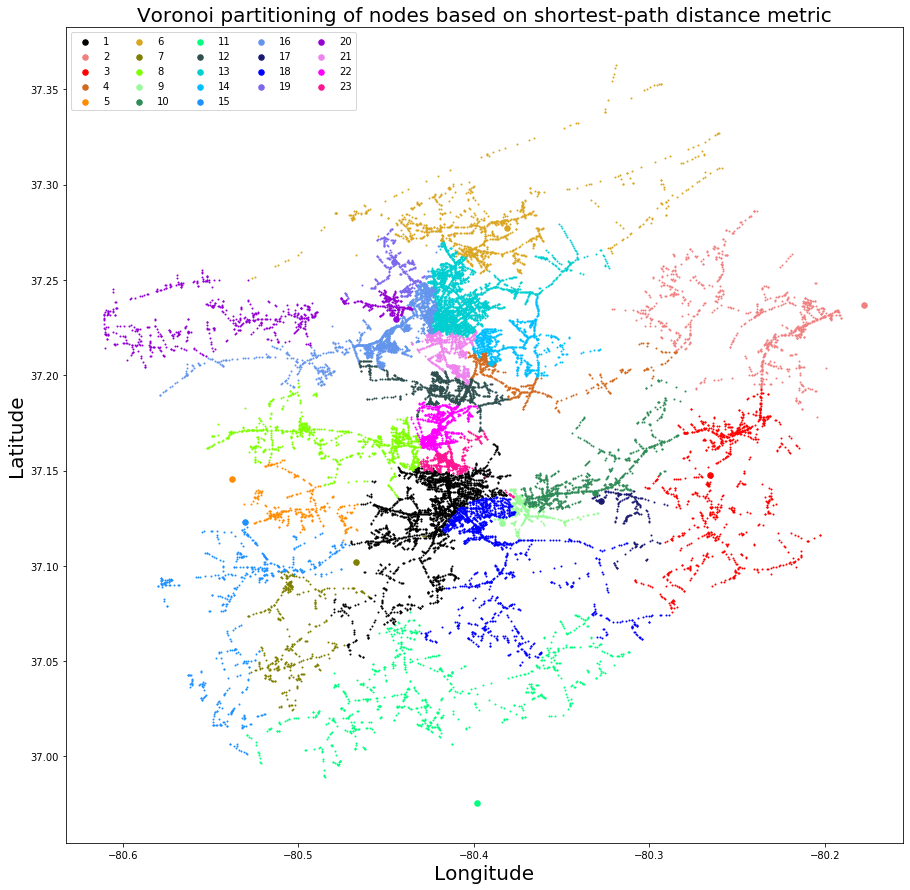
\includegraphics[width=0.48\textwidth]{figs/voronoi.png}
	\caption{Road network and transformer nodes clustered based on the shortest-path distance to different substations.}
	\label{fig:voronoi}
\end{figure}

Our goal is to identify optimal primary network $\mathcal{P}_s(\Tilde{\mathcal{V}}_s,\Tilde{\mathcal{E}}_s)$ from the set of edges in $\mathcal{G}_{s}(\mathcal{V}_s,\mathcal{E}_s)$. Note that $\mathcal{V}_s$ consists of local transformer nodes as well as road network nodes ($\mathcal{V}_s=\mathcal{V}_{s_T}\cup\mathcal{V}_{s_R}$). The optimal primary network is a forest of trees covering all nodes in the set of transformer nodes $\mathcal{V}_{s_T}$. However, not all road network nodes need to be covered as they serve as \emph{transfer} nodes which has no power consumption and are present to transfer power from preceding to succeeding node. Furthermore, the road network nodes can also act as root node connecting HV feeder lines from the substation with the primary network. That is, the nodes in set $\mathcal{V}_{s_R}$ may either be chosen to be included in $\mathcal{P}_s$ or not. If a road node is chosen it can either be a root node for a tree or can be a \emph{transfer} node with a degree of at least $2$.

\noindent\textbf{Node variables} $\mathcal{V}_s$ comprises of $n_t$ transformer and $n_r$ road nodes. Let $p_i$ denote the power consumption at the $i^{th}$ transformer node. This is obtained by summing up the total load demand of residences connected to the transformer. These power consumptions can be stacked in a $n_t$-length vector $\mathbf{p}$. Let $v_i$ represent the voltage at the node $i$. The nodal voltages at all nodes can be stacked in $n_t+n_r$ length vectors $\mathbf{v}$.

We assign binary variables $\{y_r,z_r\}_{r\in\mathcal{V}_{s_R}}\in\{0,1\}$. Variable $y_r=1$ indicates that road network node $r$ is part of the primary network and vice versa. Variable $z_r=0$ indicates that road network node $r$ is chosen and is a root node in the optimal primary network. $z_r=1$ indicates that the road node is a non-root node. Furthermore, we enforce that if a road node is not chosen ($y_r=0$), it is to be treated as a non-root node ($z_r=1$).

\noindent\textbf{Edge variables}
In order to identify which edges comprise of the primary network, each edge $e$ is assigned a binary variable $\{x_e\}_{e\in\mathcal{E}_s}\in\{0,1\}^{|\mathcal{E}_s|}$. Variable $x_e=1$ indicates that the edge is part of the optimal primary network and vice versa. The binary variable for all edges and edge power flows can be stacked in a $|\mathcal{E}_s|$-length vectors $\mathbf{x}$ and $\mathbf{f}$ respectively.

\noindent\textbf{Connectivity constraint}
The first set of constraints are defined to ensures the structural feasibility of road nodes in the optimal primary network.  
\begin{subequations}
	\begin{align}
	\sum_{e:(r,j)}&x_{e}\leq |\mathcal{E}_s|y_r,\quad \forall r\in\mathcal{V}_{s_R}\label{eq:non-chosen}\\
	\sum_{e:(r,j)}&x_{e}\geq y_r,\quad \forall r\in\mathcal{V}_{s_R}\label{eq:chosen}\\
	\sum_{e:(r,j)}&x_{e}\geq2(y_r+z_r-1),\quad \forall r\in\mathcal{V}_{s_R}\label{eq:transfer}\\
	&1-z_r\leq y_r\label{eq:non-root},\quad \forall r\in\mathcal{V}_{s_R}
	\end{align}
	\label{eq:prim-connectivity}
\end{subequations}
Let $e:(r,j)$ denote the set of all edges $e\in\mathcal{E}_s$ which are incident on the road node $r\in\mathcal{V}_{s_R}$. Therefore, $\sum_{e:(r,j)}x_{e}$ is the degree of node $r$ in graph $\mathcal{G}_s$. There are three possibilities for each road node $r$: (i) it is not chosen, (ii) it is chosen and is not a root node and (iii) it is chosen and is a root node. 

If $r$ is not chosen ($y_r=0$), (\ref{eq:non-root}) ensures $z_r=1$. (\ref{eq:non-chosen}), (\ref{eq:chosen})and (\ref{eq:transfer}) ensures that there are no incident edges on $r$. If $r$ is chosen and is a root node ($y_r=1,z_r=0$), (\ref{eq:non-chosen}), (\ref{eq:chosen})and (\ref{eq:transfer}) ensures that the degree of the road node is positive. Finally, if $r$ is chosen and is not a root node ($y_r=1,z_r=1$), it has to be a transfer node with a minimum degree of $2$ which is ensured by (\ref{eq:transfer}). The binary variables $y_r,z_r$ can be stacked in $n_r$-length vectors $\mathbf{y}$ and $\mathbf{z}$ respectively.

\noindent\textbf{Ensuring radiality constraint}
Since all the road network nodes need not be covered by the generated radial topology, we have the following equivalent of Eq.~\ref{eq:radial}.
\begin{equation}
\sum_{e\in\mathcal{E}_s}x_e=|\mathcal{V}_s|-\sum_{r\in\mathcal{V}_{s_R}}(1-y_r)-\sum_{r\in\mathcal{V}_{s_R}}(1-z_r)\label{eq:prim_radial}
\end{equation}
The total number of edges in the optimal primary network is equal to the difference between total number of nodes to be covered and number of root nodes. The last term in (\ref{eq:prim_radial}) denotes the number of root nodes and the first two terms together indicates the total number of nodes to be covered.

\noindent\textbf{Power balance and flow constraints}
We can define the branch-bus incidence matrix $\mathbf{A_{\mathcal{G}_s}}\in\mathbb{R}^{|\mathcal{V}_s|\times|\mathcal{E}_s|}$ similar to Eq.~\ref{eq:bus-incidence}. Since the order of rows and columns in $\mathbf{A_{\mathcal{G}_s}}$ is arbitrary, we can partition the rows without loss of generality as $\mathbf{A_{\mathcal{G}_s}}=\begin{bmatrix}\mathbf{A_{s_T}}^T&\mathbf{A_{s_R}}^T\end{bmatrix}^T$. Here, the partitions $\mathbf{A_{s_T}}$ and $\mathbf{A_{s_R}}$ are obtained by stacking the rows of $\mathbf{A_{\mathcal{G}_s}}$ corresponding to transformer nodes and road nodes respectively.
\begin{subequations}
	\begin{align}
	&\mathbf{A_{s_T}}\mathbf{f}=\mathbf{p}\label{eq:pf-tsfr}\\
	-&\overline{s}(1-\mathbf{z})\leq\mathbf{A_{s_R}}\mathbf{f}\leq\overline{s}(1-\mathbf{z})\label{eq:pf-road}\\
	-&\overline{f}\mathbf{x}\leq \mathbf{f}\leq \overline{f}\mathbf{x}\label{eq:pf-flow}
	\end{align}
	\label{eq:prim-pf}
\end{subequations}
(\ref{eq:pf-tsfr}) ensures that a path exists between each transformer node and a root node following Proposition~\ref{prop-1}. If a road node is not a root node (with $z_r=1$), (\ref{eq:pf-road}) enforces that the consumption at the node is $0$. If a road node is a root node (with $z_r=0$), the power consumption/injection at the node is limited by the substation power capacity limits $[-\overline{s},\overline{s}]$. (\ref{eq:pf-flow}) ensures that if an edge $e\in\mathcal{E}_s$ is selected ($x_e=1$), the power flow is limited by the line capacity limits $[-\overline{f},\overline{f}]$.

\noindent\textbf{Voltage constraints}
The long HV lines from the substation to the root nodes in the optimal primary distribution network end in voltage regulators which ensure that the root nodes have a voltage of $1$pu. This is ensured by (\ref{eq:volt-root}). (\ref{eq:volt-limit}) limits the voltage at all nodes within the acceptable limits of $[\underline{v},\overline{v}]$.
\begin{subequations}
	\begin{align}
	(1-v_r)\leq &z_r~\forall r\in\mathcal{V}_{s_R}\label{eq:volt-root}\\
	\underline{v}\mathbf{1}\leq \mathbf{v}\leq &\overline{v}\mathbf{1}\label{eq:volt-limit}\\
	-(1-x_e)M\leq &v_i-v_j-r_ef_e\leq(1-x_e)M,~\forall e\in\mathcal{E}_s\label{eq:volt-edge}
	\end{align}
	\label{eq:prim-voltage}
\end{subequations}
If $r_e$ denotes the resistance of the line $e:(i,j)\in\mathcal{E}_s$, the LDF model relates the squared voltage magnitude to power flows linearly as $v_i^2-v_j^2=2r_ef_e$ where $f_e$ is the entry from the vector $\mathbf{f}$ corresponding to edge $e$. The squared voltage can be approximated as $v_i^2\approx 2v_i-1$ which leads to the relation $v_i-v_j=r_eP_e$. Notice that this constraint is only activated for those edges $e\in\mathcal{E}_s$ for which $x_e=1$. Therefore, we can enforce this constraint as (\ref{eq:volt-edge}). If an edge is not selected ($x_e=0$), (\ref{eq:pf-flow}) ensures that $f_e=0$. Therefore, $M$ in (\ref{eq:volt-edge}) can be selected to be $M=\overline{v}-\underline{v}$.

\noindent\textbf{Generating optimal primary network} Each edge $e=(u,v)\in\mathcal{E}_s$ is assigned a weight $w_e=w(u,v)=\mathsf{dist}(u,v)$ which is the geodesic distance between the nodes. Additionally, for every road node $r\in\mathcal{V}_{s_R}$, we compute its geodesic distance from the substation $s$ and is denoted by $\mathsf{d}_r$. The optimal primary network topology is obtained by solving the optimization problem.
\begin{equation}
\begin{aligned}
\min_{\mathbf{x},\mathbf{y},\mathbf{z}}&~\sum_{e\in\mathcal{E}_s}x_ew_e+\sum_{e\in\mathcal{V}_{s_R}}(1-z_r)d_r\\
\textrm{s.to.}&~(\ref{eq:prim-connectivity}),(\ref{eq:prim_radial}),(\ref{eq:prim-pf}),(\ref{eq:prim-voltage})
\end{aligned}
\end{equation}


\begin{figure}
	\centering
	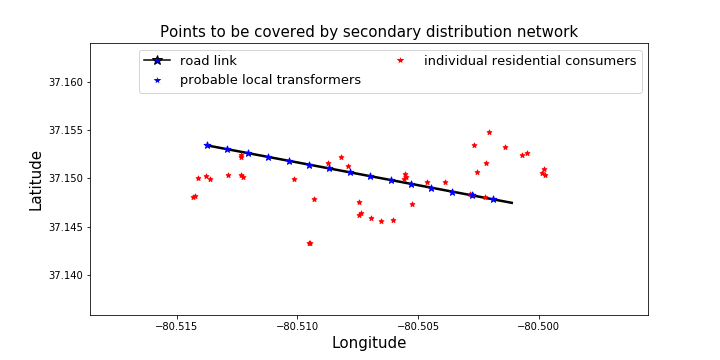
\includegraphics[width=0.48\textwidth]{figs/secnet-base.png}
	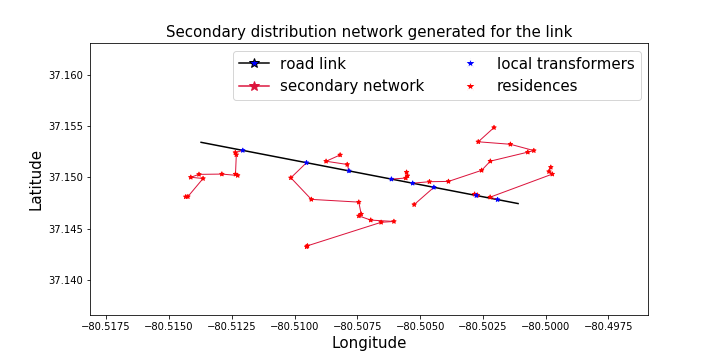
\includegraphics[width=0.48\textwidth]{figs/secnet-result.png}
	\caption{Secondary distribution network generated for a residences along a road link in Montgomery county of south-west Virginia, USA. The top figure shows the probable local transformers and residences to be connected. The bottom figure shows the generated optimal secondary distribution network.}
	\label{fig:secondary}
\end{figure}
\begin{figure*}[htb]
	\centering
	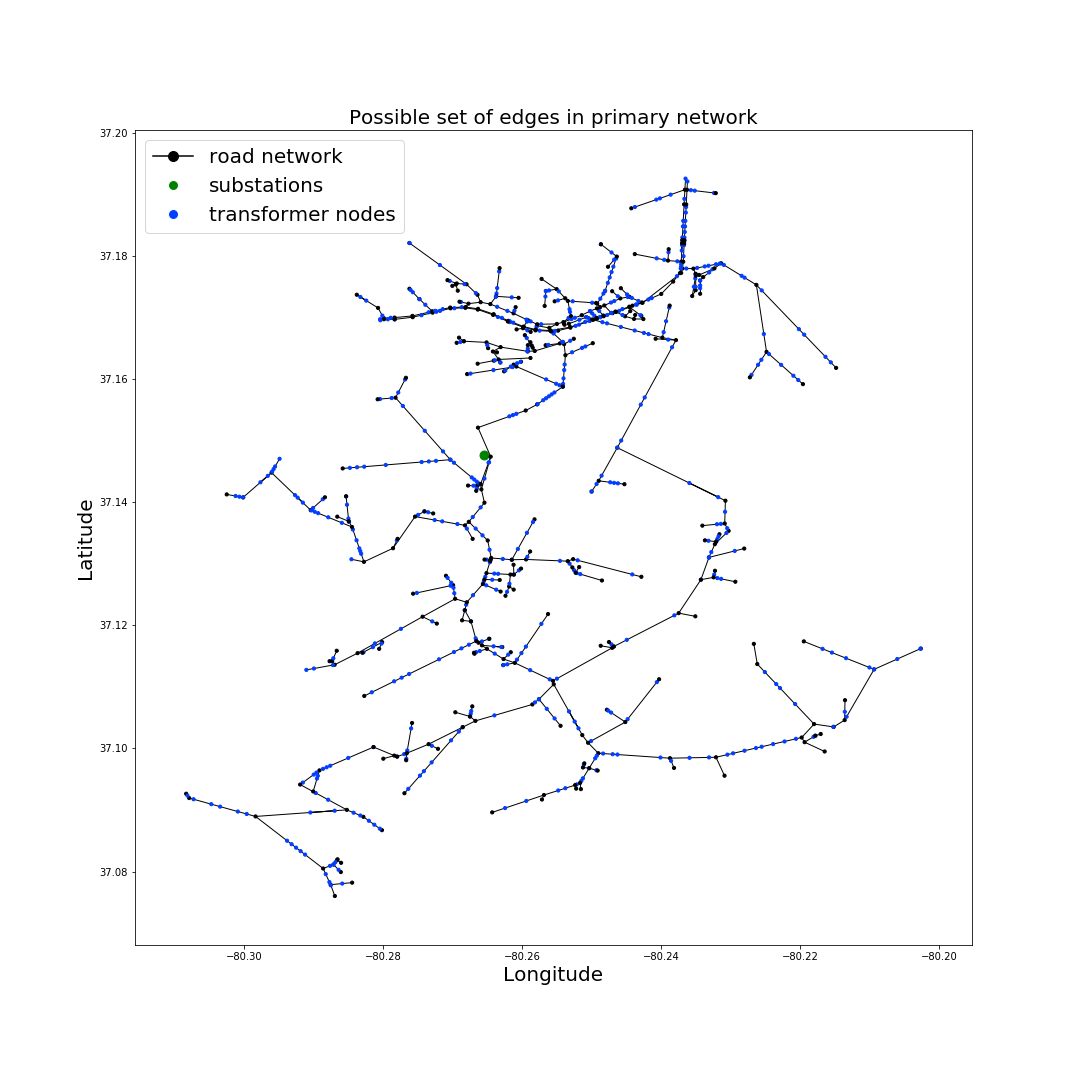
\includegraphics[width=0.47\textwidth]{figs/24664-master.png}
	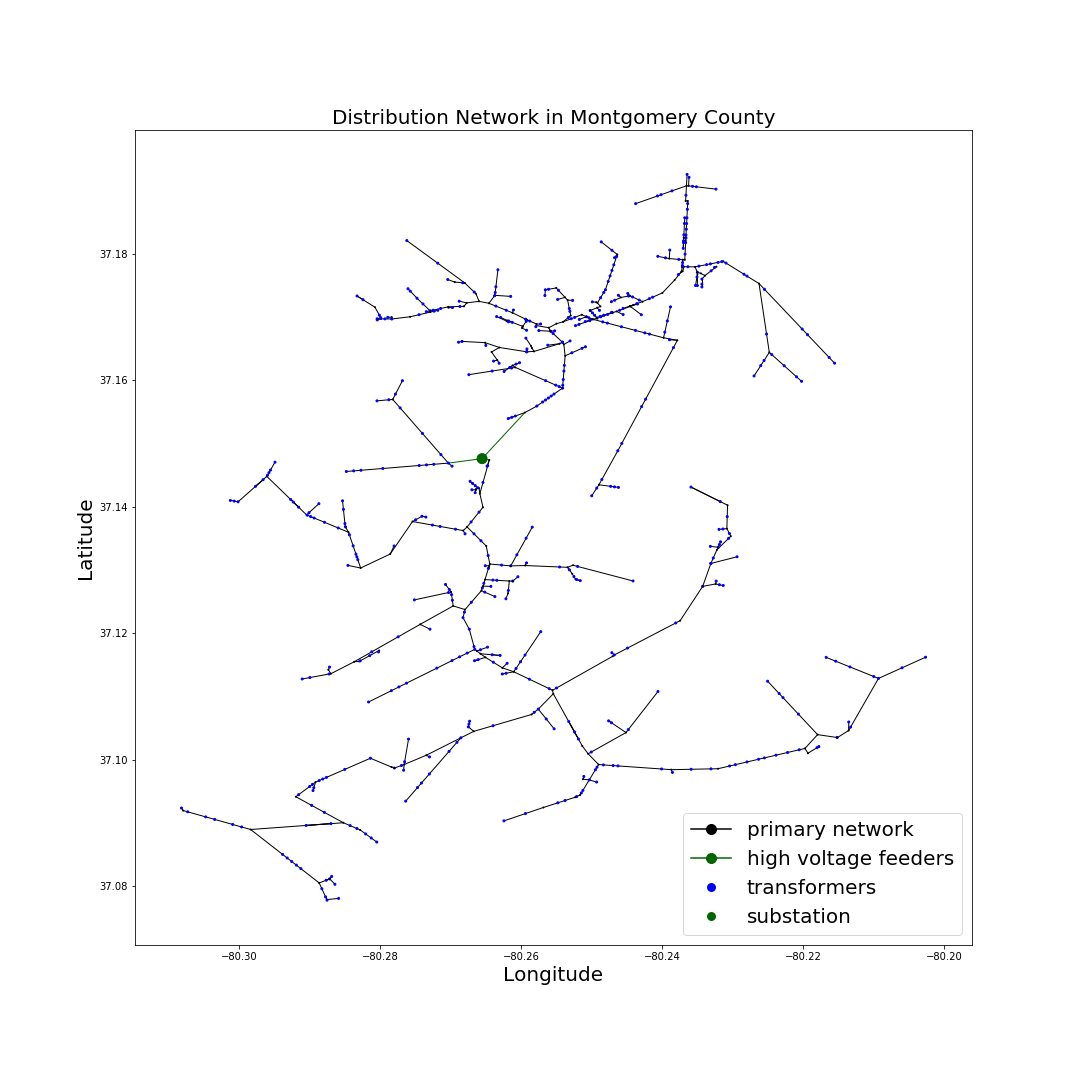
\includegraphics[width=0.47\textwidth]{figs/24664-primarytest.png}
	\caption{Primary distribution network generated for a substation in Montgomery county of south-west Virginia, USA. The left figure shows the set of possible road network edges from which the primary network is selected and the local transformers which are required to be connected. The right figure shows the optimal primary distribution with three feeders (green edges) originating from the substation.}
	\label{fig:primary}
\end{figure*}
\begin{figure*}[htb]
	\centering
	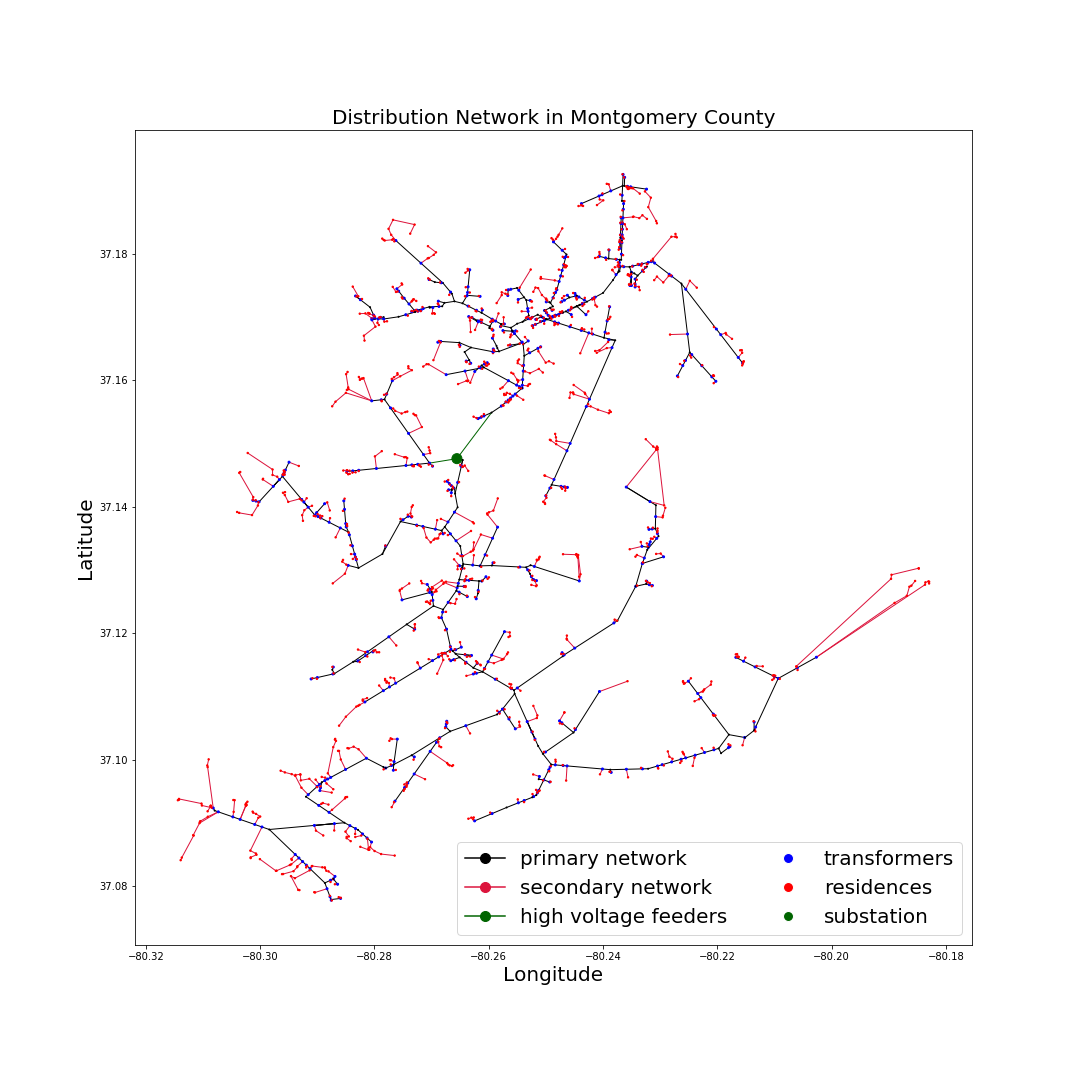
\includegraphics[width=0.45\textwidth]{figs/24664-networktest.png}
	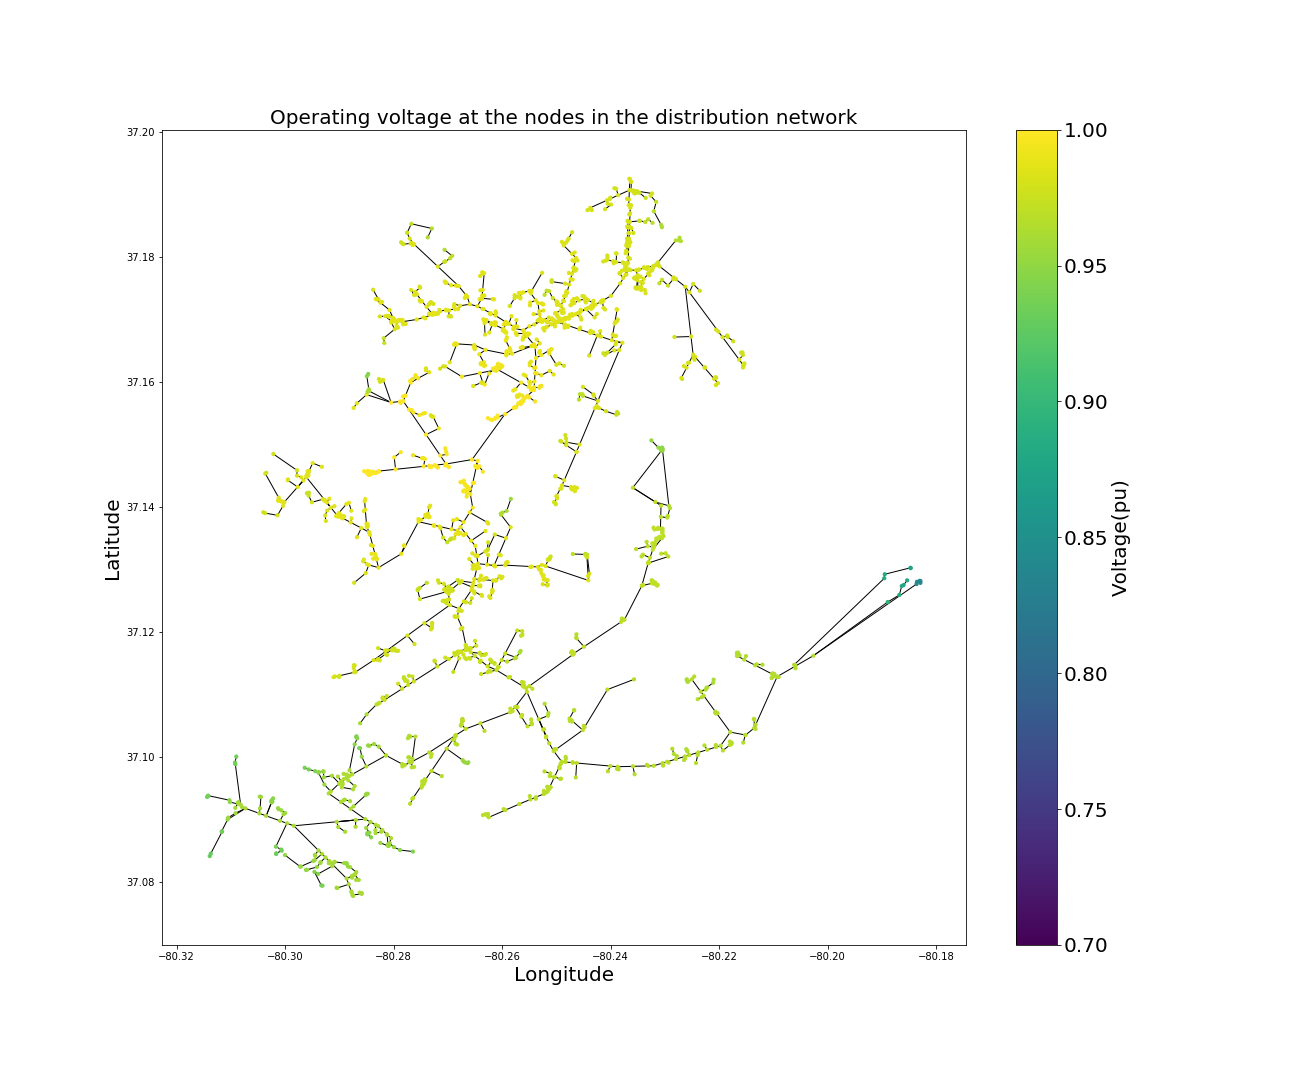
\includegraphics[width=0.535\textwidth]{figs/24664-voltagetest.png}
	\caption{The left figure shows the primary and secondary distribution network for a substation in Montgomery county of south-west Virginia, USA. The right figure shows the operating voltage at different points in the network when individual customers are consuming average load demand.}
	\label{fig:total}
\end{figure*}

\section{Results and Discussion}\label{sec:results}
The proposed methodology is used to generate synthetic distribution networks connecting substations to individual residences in Montgomery county of south-west Virginia, USA. 
\begin{table}[htb]
	\centering
	\caption{Datasets used to generate synthetic distribution network of Montgomery county}
	\label{tab:dataset}
	\begin{tabular}{@{}|c|c|c|c|@{}}
		\toprule
		Dataset & Source & Attributes & Size \\ \midrule
		\multirow{3}{*}{Substation} & \multirow{3}{*}{\begin{tabular}[c]{@{}c@{}}electric substation \\ published by \\ US Department of  \\ Homeland Security\end{tabular}} & substation ID & \multirow{3}{*}{23} \\ \cmidrule(lr){3-3}
		&  & longitude &  \\ \cmidrule(lr){3-3}
		&  & latitude &  \\ \midrule
		\multirow{5}{*}{\begin{tabular}[c]{@{}c@{}}Road \\ Network\end{tabular}} & \multirow{5}{*}{\begin{tabular}[c]{@{}c@{}}GIS and electronic \\ navigable maps \\ published by \\ NAVTEQ\end{tabular}} & road nodes & \multirow{3}{*}{8461} \\ \cmidrule(lr){3-3}
		&  & longitude &  \\ \cmidrule(lr){3-3}
		&  & latitude &  \\ \cmidrule(l){3-4} 
		&  & road links & \multirow{2}{*}{10114} \\ \cmidrule(lr){3-3}
		&  & \begin{tabular}[c]{@{}c@{}}road link \\ importance \\ level\\ (1,2,3,4,5)\end{tabular} &  \\ \midrule
		\multirow{4}{*}{Residences} & \multirow{4}{*}{\begin{tabular}[c]{@{}c@{}}synthetic \\ population and \\ electric load \\ demand profiles \\ generated by\\ ~\cite{swapna_2018}\end{tabular}} & residence ID & \multirow{4}{*}{37223} \\ \cmidrule(lr){3-3}
		&  & longitude &  \\ \cmidrule(lr){3-3}
		&  & latitude &  \\
		&  & \begin{tabular}[c]{@{}c@{}}average \\ hourly\\ load\end{tabular} &  \\ \bottomrule
	\end{tabular}
\end{table}

The first task is to map individual residential location to the nearest road network link. This is followed by the creation of secondary distribution network for each link. For example, Fig.~\ref{fig:secondary} shows the creation of secondary distribution network for a set of residences mapped to a road link. The blue points along the road link indicate the probable locations of local transformers along the link and the red points are the residences which are required to be connected. The optimal secondary network is shown in the bottom figure which covers all the residences mapped to the road link and rooted at the local transformer nodes.

The secondary network is generated for all road links mapped to at least one residence. The number of local transformers along the road links is about 14000. The final task is to generate the primary distribution network which connects these local transformers to the substations. For this purpose, we divide the entire network into separate regions as shown in Fig.~\ref{fig:voronoi}. The optimal primary network originating from one substation is shown in Fig.~\ref{fig:primary}. The first figure shows road network consisting of possible edges and the local transformers which are to be connected. The second figure shows the generated optimal primary network. Fig.~\ref{fig:total} shows the entire synthetic distribution network (primary and secondary) generated for the same substation. The generated network is validated for the structural and operational constraints. The network has a radial structure with no loops and the operating voltage at different points in the network is shown in the second figure. The operating voltages are calculated when the residential customers are consuming average load. It is observed that the voltage profile is within acceptable limits of 0.95 to 1.0 pu. The voltage profile can be further improved by optimally placing capacitors along the network.

\section{Conclusion}
This paper proposes a methodology to generate synthetic distribution networks for a particular geographical location based on available road network data. The generated network connects individual residential customers to substations while maintaining a radial configuration. Additionally, the network is created such that the overall length of overhead lines is minimized which is similar to planning methodologies undertaken by distribution companies. This ensures that generated synthetic distribution network is realistic and can be used to represent the network of the geographic location accurately. 



\bibliographystyle{abbrvnat}
\bibliography{references}
\end{document}

